% A LaTeX template for MSc Thesis submissions to 
% Politecnico di Milano (PoliMi) - School of Industrial and Information Engineering
%
% S. Bonetti, A. Gruttadauria, G. Mescolini, A. Zingaro
% e-mail: template-tesi-ingind@polimi.it
%
% Last Revision: October 2021
%
% Copyright 2021 Politecnico di Milano, Italy. NC-BY

\documentclass{Configuration_Files/PoliMi3i_thesis}

%------------------------------------------------------------------------------
%	REQUIRED PACKAGES AND  CONFIGURATIONS
%------------------------------------------------------------------------------

% CONFIGURATIONS
\usepackage{parskip} % For paragraph layout
\usepackage{setspace} % For using single or double spacing
\usepackage{emptypage} % To insert empty pages
\usepackage{multicol} % To write in multiple columns (executive summary)
\setlength\columnsep{15pt} % Column separation in executive summary
\setlength\parindent{0pt} % Indentation
\raggedbottom  

% PACKAGES FOR TITLES
\usepackage{titlesec}
% \titlespacing{\section}{left spacing}{before spacing}{after spacing}
\titlespacing{\section}{0pt}{3.3ex}{2ex}
\titlespacing{\subsection}{0pt}{3.3ex}{1.65ex}
\titlespacing{\subsubsection}{0pt}{3.3ex}{1ex}
\usepackage{color}

% PACKAGES FOR LANGUAGE AND FONT
\usepackage[english]{babel} % The document is in English  
\usepackage[utf8]{inputenc} % UTF8 encoding
\usepackage[T1]{fontenc} % Font encoding
\usepackage[11pt]{moresize} % Big fonts

% PACKAGES FOR IMAGES
\usepackage{graphicx}
\usepackage{transparent} % Enables transparent images
\usepackage{eso-pic} % For the background picture on the title page
\usepackage{subfig} % Numbered and caption subfigures using \subfloat.
\usepackage{tikz} % A package for high-quality hand-made figures.
\usetikzlibrary{}
\graphicspath{{./Images/}} % Directory of the images
\usepackage{caption} % Coloured captions
\usepackage{xcolor} % Coloured captions
\usepackage{amsthm,thmtools,xcolor} % Coloured "Theorem"
\usepackage{float}

% STANDARD MATH PACKAGES
\usepackage{amsmath}
\usepackage{amsthm}
\usepackage{amssymb}
\usepackage{amsfonts}
\usepackage{bm}
\usepackage[overload]{empheq} % For braced-style systems of equations.
\usepackage{fix-cm} % To override original LaTeX restrictions on sizes

% PACKAGES FOR TABLES
\usepackage{tabularx}
\usepackage{longtable} % Tables that can span several pages
\usepackage{colortbl}

% PACKAGES FOR ALGORITHMS (PSEUDO-CODE)
\usepackage{algorithm}
\usepackage{algorithmic}

% PACKAGES FOR REFERENCES & BIBLIOGRAPHY
\usepackage[colorlinks=true,linkcolor=black,anchorcolor=black,citecolor=black,filecolor=black,menucolor=black,runcolor=black,urlcolor=black]{hyperref} % Adds clickable links at references
\usepackage{cleveref}
\usepackage[square, numbers, sort&compress]{natbib} % Square brackets, citing references with numbers, citations sorted by appearance in the text and compressed
\bibliographystyle{abbrvnat} % You may use a different style adapted to your field

% OTHER PACKAGES
\usepackage{pdfpages} % To include a pdf file
\usepackage{afterpage}
\usepackage{lipsum} % DUMMY PACKAGE
\usepackage{fancyhdr} % For the headers
\fancyhf{}

% Input of configuration file. Do not change config.tex file unless you really know what you are doing. 
% Define blue color typical of polimi
\definecolor{bluepoli}{cmyk}{0.4,0.1,0,0.4}

% Custom theorem environments
\declaretheoremstyle[
  headfont=\color{bluepoli}\normalfont\bfseries,
  bodyfont=\color{black}\normalfont\itshape,
]{colored}

% Set-up caption colors
\captionsetup[figure]{labelfont={color=bluepoli}} % Set colour of the captions
\captionsetup[table]{labelfont={color=bluepoli}} % Set colour of the captions
\captionsetup[algorithm]{labelfont={color=bluepoli}} % Set colour of the captions

\theoremstyle{colored}
\newtheorem{theorem}{Theorem}[chapter]
\newtheorem{proposition}{Proposition}[chapter]

% Enhances the features of the standard "table" and "tabular" environments.
\newcommand\T{\rule{0pt}{2.6ex}}
\newcommand\B{\rule[-1.2ex]{0pt}{0pt}}

% Pseudo-code algorithm descriptions.
\newcounter{algsubstate}
\renewcommand{\thealgsubstate}{\alph{algsubstate}}
\newenvironment{algsubstates}
  {\setcounter{algsubstate}{0}%
   \renewcommand{\STATE}{%
     \stepcounter{algsubstate}%
     \Statex {\small\thealgsubstate:}\space}}
  {}

% New font size
\newcommand\numfontsize{\@setfontsize\Huge{200}{60}}

% Title format: chapter
\titleformat{\chapter}[hang]{
\fontsize{50}{20}\selectfont\bfseries\filright}{\textcolor{bluepoli} \thechapter\hsp\hspace{2mm}\textcolor{bluepoli}{|   }\hsp}{0pt}{\huge\bfseries \textcolor{bluepoli}
}

% Title format: section
\titleformat{\section}
{\color{bluepoli}\normalfont\Large\bfseries}
{\color{bluepoli}\thesection.}{1em}{}

% Title format: subsection
\titleformat{\subsection}
{\color{bluepoli}\normalfont\large\bfseries}
{\color{bluepoli}\thesubsection.}{1em}{}

% Title format: subsubsection
\titleformat{\subsubsection}
{\color{bluepoli}\normalfont\large\bfseries}
{\color{bluepoli}\thesubsubsection.}{1em}{}

% Shortening for setting no horizontal-spacing
\newcommand{\hsp}{\hspace{0pt}}

\makeatletter
% Renewcommand: cleardoublepage including the background pic
\renewcommand*\cleardoublepage{%
  \clearpage\if@twoside\ifodd\c@page\else
  \null
  \AddToShipoutPicture*{\BackgroundPic}
  \thispagestyle{empty}%
  \newpage
  \if@twocolumn\hbox{}\newpage\fi\fi\fi}
\makeatother

%For correctly numbering algorithms
\numberwithin{algorithm}{chapter}

%----------------------------------------------------------------------------
%	NEW COMMANDS DEFINED
%----------------------------------------------------------------------------

% EXAMPLES OF NEW COMMANDS
\newcommand{\bea}{\begin{eqnarray}} % Shortcut for equation arrays
\newcommand{\eea}{\end{eqnarray}}
\newcommand{\e}[1]{\times 10^{#1}}  % Powers of 10 notation

%----------------------------------------------------------------------------
%	ADD YOUR PACKAGES (be careful of package interaction)
%----------------------------------------------------------------------------
\usepackage{listings}
\usepackage{xcolor}
\usepackage{geometry}

\lstdefinelanguage{MongoDB}{
  morekeywords={db, aggregate, \$group, \$bucket, \$match, \_id, \$max, \$avg, \$sum, \$first, \$sort, \$limit, sort, \$project, \$cond, if, then, else},
  sensitive=true,
  morecomment=[l]{//},
  morecomment=[s]{/*}{*/},
  morestring=[b]'"
}

\lstset{
  language=MongoDB,
  basicstyle=\ttfamily,
  keywordstyle=\color{blue},
  commentstyle=\color{green!40!black},
  stringstyle=\color{black},
  stepnumber=1,
  numberstyle=\tiny\color{gray},
  breaklines=true,
  breakatwhitespace=true,
  tabsize=4
}

%----------------------------------------------------------------------------
%	ADD YOUR DEFINITIONS AND COMMANDS (be careful of existing commands)
%----------------------------------------------------------------------------

%----------------------------------------------------------------------------
%	BEGIN OF YOUR DOCUMENT
%----------------------------------------------------------------------------

\begin{document}

\fancypagestyle{plain}{%
\fancyhf{} % Clear all header and footer fields
\fancyhead[RO,RE]{\thepage} %RO=right odd, RE=right even
\renewcommand{\headrulewidth}{0pt}
\renewcommand{\footrulewidth}{0pt}}

%----------------------------------------------------------------------------
%	TITLE PAGE
%----------------------------------------------------------------------------

\pagestyle{empty} % No page numbers
\frontmatter % Use roman page numbering style (i, ii, iii, iv...) for the preamble pages

\puttitle{
	title=Systems and Methods for Big and Unstructured Data Project,
	name1=Matteo Balice (10978268), % Author Name and Surname
	name2=Antonio Giuseppe Doronzo (11016435), 
	name3=Alessandro Masini (10940986), 
	name4=,
	name5=,
	academicyear=2023-2024
	%groupnumber=
} % These info will be put into your Title page 

%----------------------------------------------------------------------------
%	PREAMBLE PAGES: ABSTRACT (inglese e italiano), EXECUTIVE SUMMARY
%----------------------------------------------------------------------------
\startpreamble
\setcounter{page}{1} % Set page counter to 1

%----------------------------------------------------------------------------
%	LIST OF CONTENTS/FIGURES/TABLES/SYMBOLS
%----------------------------------------------------------------------------

% TABLE OF CONTENTS
\thispagestyle{empty}
\tableofcontents % Table of contents 
\thispagestyle{empty}
\cleardoublepage

%-------------------------------------------------------------------------
%	THESIS MAIN TEXT
%-------------------------------------------------------------------------
% In the main text of your thesis you can write the chapters in two different ways:
%
%(1) As presented in this template you can write:
%    \chapter{Title of the chapter}
%    *body of the chapter*
%
%(2) You can write your chapter in a separated .tex file and then include it in the main file with the following command:
%    \chapter{Title of the chapter}
%    \input{chapter_file.tex}
%
% Especially for long thesis, we recommend you the second option.

\addtocontents{toc}{\vspace{2em}} % Add a gap in the Contents, for aesthetics
\mainmatter % Begin numeric (1,2,3...) page numbering



\chapter{MongoDB}
\label{ch:chapter_one}%
% The \label{...}% enables to remove the small indentation that is generated, always leave the % symbol.

\section{Introduction}
Using the following dataset we'd like to tackle the problem of researching whether songs of the same genre also share specific values of the main features describing them (for example the energy or the danceability) and whether tracks with certain features are more likely to become popular than others.\\
To face such task a documental database technology (more specifically MongoDB) has been chosen, since in this dataset the relationship between each object is quite often not relevant, and we care much more about the features of each single track, furthermore the granularity to which we'd like to operate is always the one of the single track, which therefore fit as a perfect business object for our day-to-day activity.
\newpage

\section{Dataset}
This dataset provides comprehensive information about tracks available on the Spotify application, each document represent a single track that can be easily found by searching its name through Spotify search feature.\\
The data schema is:
\begin{table}[h!]
	\begin{center}
		\begin{tabular}{|m{12em}|m{4em}|m{25em}|}
		\hline
		\textbf{Attribute} & \textbf{Type} & \textbf{Description}\\
		\hline
			track\_id & String & The song unique ID\\
		\hline
			track\_name & String & The name of the track\\
		\hline
			track\_artist & String & The name of the artist that made the song\\
		\hline
			track\_popularity & Integer & The popularity score of the track on Spotify ranging from a minimum of 0 to a maximum of 100.\\
		\hline
			track\_album\_id & String & The unique ID of the album\\
		\hline
			track\_album\_name & String & The name of the album the track belongs to\\
		\hline
			track\_album\_release\_date & Date & The date in which the album was released\\
		\hline
			playlist\_name & String & The name of the playlist in which Spotify classified this song\\
		\hline
			playlist\_id & String & The ID of the playlist in which Spotify classified this song\\
		\hline
			playlist\_genre & String & The genre of the playlist in which Spotify classified this song\\
		\hline
			playlist\_subgenre & String & The subgenre of the playlist in which Spotify classified this song\\
		\hline
			danceability & Double & A score ranging from 0 to 1 that represents how suitable a track is for dancing based on various musical elements including tempo, rhythm stability, beat strength, and overall regularity.\\
		\hline
			energy & Double & A measure of the perceptual intensity and activity of a track, ranging from 0 to 1. Typically, energetic tracks feel fast, loud, and noisy. For example, death metal's tracks have high energy, while a Bach prelude scores low on this scale.\\
		\hline
			key & Integer & The estimated overall key of the track. Standard integer pitch notation is used, e.g. C = 0, C$\sharp$/D$\flat$ = 1, D = 2, and so on, while if no key was detected, a value of -1 is assigned\\
		\hline
		\end{tabular}
	\end{center}
\end{table}\newpage

\begin{table}[h!]
	\begin{center}
		\hspace*{-1cm}
		\begin{tabular}{|m{8em}|m{4em}|m{29em}|}
		\hline
		\textbf{Attribute} & \textbf{Type} & \textbf{Description}\\
		\hline
			loudness & Double & The overall loudness of a track in decibels (dB). Loudness values are averaged across the entire track and typically range between -60 and 0 db\\
		\hline
			mode & Integer & The tonal mode of the track, the type of scale from which its melodic content is derived, represented by an integer value (0 for minor, 1 for major).\\
		\hline
			speechiness & Double & A score ranging from 0 to 1 that represents the presence of spoken words in a track. The more exclusively speech-like the recording the closer to 1.0 the attribute value.\\
		\hline
			acousticness & Double & A score ranging from 0 to 1 that represents the confidence of a track being acoustic or similarly the extent to which a track possesses an acoustic quality. (1.0 represents very high confidence that the track is acoustic)\\
		\hline
			instrumentalness & Double & A score ranging from 0 to 1 that represents the likelihood of a track being instrumental (so having no vocals). The closer the instrumentalness value is to 1.0, the greater is the likelihood that the track contains no vocal content, values above 0.5 can be considered as instrumental tracks, but confidence is higher as the value approaches 1.0.\\
		\hline
			liveness & Double & A score ranging from 0 to 1 that represents the probability of the presence of an audience during the recording or performance of a track. A value above 0.8 provides a strong likelihood that the track has been performed live.\\
		\hline
			valence & Double & A score ranging from 0 to 1 that represents the musical positiveness conveyed by a track. Tracks with high valence sound more positive (happy, cheerful, euphoric), while tracks with low valence sound more negative (sad, depressed, angry).\\
		\hline
			tempo & Double & The overall estimated tempo of the track in beats per minute (BPM). Tempo is perceived as the speed or pace of a given track.\\
		\hline
			duration\_ms & Integer & The duration of the track in milliseconds.\\
		\hline
		\end{tabular}
		\hspace*{1cm}
	\end{center}
\end{table}
The source of the dataset is:\\
\url{https://www.kaggle.com/datasets/joebeachcapital/30000-spotify-songs}
\newpage
\section*{Queries}
\subsection{Preferred musical genre}
This query analyses the popularity of each musical genre, by calculating the average of the track\_popularity score for each one of them, in order to understand what musical genre are the user's favorites\\

\begin{algorithm}[ht]
\caption{Preferred musical genre}
\begin{lstlisting} [numbers = left]
db.spotify_music.aggregate([
	{"$group" : {
			"_id" : {"Music_genre" : "$playlist_genre"},
			"Popularity" : {"$avg" : "$track_popularity"},
			"Number_of_samples" : {"$sum" : 1}
	}}
]).sort({
	"Popularity" : -1
})
\end{lstlisting}
\end{algorithm}
\newpage

Output:
\begin{algorithm}[h!]
\caption{Output Preferred musical genre}
\begin{lstlisting} [numbers = left]
[
	{
		_id: { Music_genre: 'pop' },
		Popularity: 47.74487016524424,
		Number_of_samples: 5507
	},
	{
		_id: { Music_genre: 'latin' },
		Popularity: 47.026576139670226,
		Number_of_samples: 5155
	},
	{
		_id: { Music_genre: 'rap' },
		Popularity: 43.21545422902889,
		Number_of_samples: 5746
	},
	{
		_id: { Music_genre: 'rock' },
		Popularity: 41.72833770955363,
		Number_of_samples: 4951
	},
	{
		_id: { Music_genre: 'r&b' },
		Popularity: 41.22353157797827,
		Number_of_samples: 5431
	},
	{
		_id: { Music_genre: 'edm' },
		Popularity: 34.83352639417508,
		Number_of_samples: 6043
	}
]
\end{lstlisting}
\end{algorithm}
\newpage

\subsection{Most popular song for each genre}
This query explores which is the most popular song in each genre, by finding the song with the highest popularity score among each one of them (we have chosen for this query to allow songs to be in more than one genre, if they have been classified as such)\\
\begin{algorithm}[ht]
\caption{Most popular song for each genre}
\begin{lstlisting} [numbers = left]
db.spotify_music.aggregate([
	{$group: {
		_id: "$playlist_genre",
		Most_Popular_Song: {
			$max: {
				Popularity: "$track_popularity",
				Title: "$track_name",
				Artist: "$track_artist"
			}
		}
	}},
	{"$sort" : {"_id" : 1}}
])
\end{lstlisting}
\end{algorithm}
\newpage

\newgeometry{top = 8 em}
\begin{algorithm}[ht]
\caption{Output: Most popular song for each genre}
\begin{lstlisting} [numbers = left]
[
	{
		_id: 'edm',
		Most_Popular_Song: {
			Popularity: 99,
			Title: 'ROXANNE',
			Artist: 'Arizona Zervas' 
		}
	},
	{
		_id: 'latin',
		Most_Popular_Song: {
			Popularity: 100,
			Title: 'Dance Monkey',
			Artist: 'Tones and I'
		}
	},
	{
		_id: 'pop',
		Most_Popular_Song: {
			Popularity: 100,
			Title: 'Dance Monkey',
			Artist: 'Tones and I' 
		}
	},
	{
		_id: 'r&b',
		Most_Popular_Song: {
			Popularity: 99,
			Title: 'ROXANNE',
			Artist: 'Arizona Zervas'
		}
	},
	{
		_id: 'rap',
		Most_Popular_Song: {
			Popularity: 98,
			Title: 'Tusa',
			Artist: 'KAROL G'
		}
	},
	{
		_id: 'rock',
		Most_Popular_Song: {
			Popularity: 95,
			Title: 'bad guy',
			Artist: 'Billie Eilish'
		}
	}
]
\end{lstlisting}
\end{algorithm}
\restoregeometry

\subsection{Loudest musical genre}
This query tries to understand which are the three loudest musical genre, by calculating the average loudness of each one of them and then showing the loudest three as output\\

\begin{algorithm}[ht]
\caption{Loudest musical genre}
\begin{lstlisting} [numbers = left]
	db.spotify_music.aggregate([
		{"$group" : {
			  "_id" : {"Music_genre" : "$playlist_genre"},
			  "Average_loudness" : {"$avg" : "$loudness"},
			  "Number_of_samples" : {"$sum" : 1}
		}},
  		{"$sort" : {"Average_loudness" : -1}},
    	{"$limit" : 3}
	])
\end{lstlisting}
\end{algorithm}
\newpage

Output:
\begin{algorithm}[ht]
\caption{Output: Loudest musical genre}
\begin{lstlisting} [numbers = left]
[
	{
		_id: { Music_genre: 'edm' },
		Average_loudness: -5.427445143140824,
		Number_of_samples: 6043
	},
	{
		_id: { Music_genre: 'latin' },
		Average_loudness: -6.264454704170708,
		Number_of_samples: 5155
	},
	{
		_id: { Music_genre: 'pop' },
		Average_loudness: -6.315328127837298,
		Number_of_samples: 5507
	}
]
\end{lstlisting}
\end{algorithm}
\newpage

\subsection{Most danceable musical genre}
This query explores which musical genre are the most danceable, by calculating the average danceability of each one of them\\
\begin{algorithm}[ht]
\caption{Most danceable musical genre}
\begin{lstlisting} [numbers = left]
db.spotify_music.aggregate([
	{"$group" : {
		"_id" : {"Music_genre" : "$playlist_genre"},
		"Average_danceability" : {"$avg" : "$danceability"},
		"Number_of_samples" : {"$sum" : 1}
	}},
  	{"$sort" : {"Average_danceability" : -1}}
])
\end{lstlisting}
\end{algorithm}
\newpage

Output:
\begin{algorithm}[ht]
\caption{Output: Most danceable musical genre}
\begin{lstlisting} [numbers = left]
[
	{
		_id: { Music_genre: 'rap' },
		Average_danceability: 0.7183527671423598,
		Number_of_samples: 5746
	},
	{
		_id: { Music_genre: 'latin' },
		Average_danceability: 0.7132872550921435,
		Number_of_samples: 5155
	},
	{
		_id: { Music_genre: 'r&b' },
		Average_danceability: 0.6701793408212116,
		Number_of_samples: 5431
	},
	{
		_id: { Music_genre: 'edm' },
		Average_danceability: 0.6550408737382095,
		Number_of_samples: 6043
	},
	{
		_id: { Music_genre: 'pop' },
		Average_danceability: 0.6393017069184674,
		Number_of_samples: 5507
	},
	{
		_id: { Music_genre: 'rock' },
		Average_danceability: 0.5205479701070491,
		Number_of_samples: 4951
	}
]
\end{lstlisting}
\end{algorithm}
\newpage
\subsection{Most popular artists}
This query analyses the popularity of each musical artist, by calculating the average between the track\_popularity score of each one of their songs for each artist, in order to understand which artists produce musical hits more consistently.\\
For this query, only artist that have produced at least two different songs have been considered
\begin{algorithm}[ht]
\caption{Most popular artists}
\begin{lstlisting} [numbers = left]
db.spotify_music.aggregate([
	{"$group" : {
			"_id" : {"track_id" : "$track_id"},
			"track_artist" : {"$first" : "$track_artist"}, 
			"track_popularity" : {"$max" : "$track_popularity"}
	}},
	{"$group" : {
		"_id" : {"Track_Artist" : "$track_artist"},
		"Average_Song_Popularity" : {"$avg" : "$track_popularity"},
		"Number_of_Songs" : {"$sum" : 1}
	}},
	{"$match" : {"Number_of_Songs" : {"$gte" : 2}}},
	{"$sort" : {"Average_Song_Popularity" : -1}},
	{"$limit" : 7}
])
\end{lstlisting}
\end{algorithm}
\newpage

Output:
\begin{algorithm}[h!]
\caption{Output: Most popular artists}
\begin{lstlisting} [numbers = left]
[
	{
		_id: { Track_Artist: 'Don Toliver' },
		Average_Song_Popularity: 87.5,
		Number_of_Songs: 2
	},
	{
		_id: { Track_Artist: 'Kina' },
		Average_Song_Popularity: 85.5,
		Number_of_Songs: 2
	},
	{
		_id: { Track_Artist: 'JACKBOYS' },
		Average_Song_Popularity: 84.33333333333333,
		Number_of_Songs: 3
	},
	{
		_id: { Track_Artist: 'DaBaby' },
		Average_Song_Popularity: 83.66666666666667,
		Number_of_Songs: 6
	},
	{
		_id: { Track_Artist: 'Roddy Ricch' },
		Average_Song_Popularity: 83.42857142857143,
		Number_of_Songs: 7
	},
	{
		_id: { Track_Artist: 'Harry Styles' },
		Average_Song_Popularity: 81.77777777777777,
		Number_of_Songs: 9
	},
	{
		_id: { Track_Artist: 'YNW Melly' },
		Average_Song_Popularity: 81.57142857142857,
		Number_of_Songs: 7
	}
]
\end{lstlisting}
\end{algorithm}
\newpage

\subsection{Most popular albums}
This query explores what are the most popular albums on Spotify at the moment, by calculating the average of the track\_popularity score among each of their songs.\\
For this query, only albums for which we have data on at least three different tracks are considered
\begin{algorithm}[ht]
\caption{Most popular albums}
\begin{lstlisting} [numbers = left]
db.spotify_music.aggregate([
	{"$group" : {
		"_id" : {"track_id" : "$track_id" },
		"track_artist" : {"$first" : "$track_artist"},
		"track_popularity" : {"$max" : "$track_popularity"},
		"track_album_id" : {"$first" : "$track_album_id"},
		"track_album_name" : {"$first" : "$track_album_name"}
	}},
	{"$group" : {
		"_id" : { "Album_id" : "$track_album_id" },
		"Artist" : {"$first" : "$track_artist"},
		"Album_Name" : {"$first" : "$track_album_name"},
		"Average_Song_Popularity" : {"$avg" : "$track_popularity"},
		"Number_of_Songs" : {"$sum" : 1}
	}},
	{"$match" : {"Number_of_Songs" : {"$gte" : 3}}},
	{"$sort" : {"Average_Song_Popularity" : -1}},
	{"$limit" : 5}
])
\end{lstlisting}
\end{algorithm}
\newpage

\newgeometry{top = 5 em}
Output:
\begin{algorithm}[h!]
\caption{Output: Most popular albums}
\begin{lstlisting} [numbers = left]
[
	{
		_id: { Album_id: '4g1ZRSobMefqF6nelkgibi' },
		Artist: 'Post Malone',
		Album_Name: "Hollywood's Bleeding",
		Average_Song_Popularity: 90.5,
		Number_of_Songs: 4
	},
	{
		_id: { Album_id: '1NsTSXjVNE7XmZ8PmyW0wl' },
		Artist: 'DaBaby',
		Album_Name: 'KIRK',
		Average_Song_Popularity: 89,
		Number_of_Songs: 3
	},
	{
		_id: { Album_id: '7xV2TzoaVc0ycW7fwBwAml' },
		Artist: 'Harry Styles',
		Album_Name: 'Fine Line',
		Average_Song_Popularity: 87.33333333333333,
		Number_of_Songs: 3
	},
	{
		_id: { Album_id: '52u4anZbHd6UInnmHRFzba' },
		Artist: 'Roddy Ricch',
		Album_Name: 'Please Excuse Me For Being Antisocial',
		Average_Song_Popularity: 86.25,
		Number_of_Songs: 4
	},
	{
		_id: { Album_id: '6tkjU4Umpo79wwkgPMV3nZ' },
		Artist: 'Juice WRLD',
		Album_Name: 'Goodbye & Good Riddance',
		Average_Song_Popularity: 85.5,
		Number_of_Songs: 4
	}
]
\end{lstlisting}
\end{algorithm}
\newpage
\restoregeometry

\subsection{Longest tracks}
In this query we search for the longest tracks in the whole dataset\\
The duration of each song has been converted into minutes for readability purposes\\
\begin{algorithm}[ht]
\caption{Longest tracks}
\begin{lstlisting} [numbers = left]
db.spotify_music.aggregate([
	{"$group" : {
		"_id" : {"Track_id" : "$track_id" },
		"Track_Name" : {"$first" : "$track_name"},
		"Track_Artist" : {"$first" : "$track_artist"},
		"Duration_min" : {"$max" : {"$divide" : ["$duration_ms", 60000]}}
	}},
	{"$sort" : {"Duration_min" : -1}},
	{"$limit": 5}
])
\end{lstlisting}
\end{algorithm}
\newpage

Output:
\begin{algorithm}[h!]
\caption{Output: Longest tracks}
\begin{lstlisting} [numbers = left]
[
	{
		_id: { Track_id: '6IoKSUyNOOheJRjiuGb1ew' },
		Track_Name: '47 - Remix',
		Track_Artist: 'Anuel AA',
		Duration_min: 8.630166666666666
	},
	{
		_id: { Track_id: '6Vjk8MNXpQpi0F4BefdTyq' },
		Track_Name: 'Kashmir - 2012 Remaster',
		Track_Artist: 'Led Zeppelin',
		Duration_min: 8.61875
	},
	{
		_id: { Track_id: '1fDsrQ23eTAVFElUMaf38X' },
		Track_Name: 'American Pie',
		Track_Artist: 'Don McLean',
		Duration_min: 8.614883333333333
	},
	{
		_id: { Track_id: '22Nq8jG98vSGghSyBsIjMO' },
		Track_Name: 'Jam On It (Re-Recorded Version)',
		Track_Artist: 'Newcleus',
		Duration_min: 8.612666666666666
	},
	{
		_id: { Track_id: '7lPjS6Yd4lRk4BsboDsm1H' },
		Track_Name: 'Roundabout - 2008 Remaster',
		Track_Artist: 'Yes',
		Duration_min: 8.599333333333334
	}
]
\end{lstlisting}
\end{algorithm}
\newpage

\subsection{What tempo is more popular?}
This query analyses what range of values for the tempo is preferred by artists, and if there is a certain tempo range that is also generally preferred by users\\
The selected tempo ranges are:
\begin{itemize}
	\item 0 $\le x_{tempo} <$ 75
	\item 75 $\le x_{tempo} <$ 100
	\item 100 $\le x_{tempo} <$ 125
	\item 125 $\le x_{tempo} <$ 150
	\item 150 $\le x_{tempo} <$ 175
	\item 175 $\le x_{tempo} <$ 250
\end{itemize}

\begin{algorithm}[ht]
\caption{What tempo is more popular?}
\begin{lstlisting} [numbers = left]
db.spotify_music.aggregate([
	{"$group" : {
			"_id" : {"Track_id" : "$track_id"},
			"tempo" : {"$first" : "$tempo"},
			"track_popularity" : {"$first" : "$track_popularity"},
	}},
	{$bucket: {
		groupBy: "$tempo",
		boundaries: [0, 75, 100, 125, 150, 175, 250],
		default: "Other",
		output: {
			"Average_popularity": { $avg: "$track_popularity" },
			"Number_of_samples": { $sum: 1 }
		}
	}}
])
\end{lstlisting}
\end{algorithm}
\newpage

Output:
\begin{algorithm}[ht]
\caption{Output: What tempo is more popular?}
\begin{lstlisting} [numbers = left]
[
	{
		_id: 0,
		Average_popularity: 40.631147540983605,
		Number_of_samples: 366
	},
	{
		_id: 75,
		Average_popularity: 40.434599156118146,
		Number_of_samples: 6873
	},
	{
		_id: 100,
		Average_popularity: 39.97265987025023,
		Number_of_samples: 8632
	},
	{
		_id: 125,
		Average_popularity: 36.618880710363364,
		Number_of_samples: 8559
	},
	{
		_id: 150,
		Average_popularity: 41.83413908516177,
		Number_of_samples: 2689
	},
	{
		_id: 175,
		Average_popularity: 41.63298302344381,
		Number_of_samples: 1237
	}
]
\end{lstlisting}
\end{algorithm}

\newpage

\subsection{Average valence of each genre}
This query analyses the valence of each musical genre, by calculating the average, in order to understand what musical genres are the most positive.\\

\begin{algorithm}[ht]
\caption{Valence of each genre}
\begin{lstlisting} [numbers = left]
db.spotify_music.aggregate([
	{ $group: {
        "_id": "$playlist_genre",
        "avg_valence": { $avg: "$valence" }
     } 
]).sort({
	"avg_valence" : -1
})
\end{lstlisting}
\end{algorithm}
\newpage

Output:
\begin{algorithm}[h!]
\caption{Output valence of each genre}
\begin{lstlisting} [numbers = left]
[
	{
      "_id": "latin",
      "avg_valence": 0.6055104267701261
    },
	{
      "_id": "rock",
      "avg_valence": 0.5373520500908907
    },
	{
      "_id": "r&b",
      "avg_valence": 0.531230602099061
    },
	{
      "_id": "rap",
      "avg_valence": 0.5050900104420466
    },
	{
      "_id": "pop",
      "avg_valence": 0.5035210277828218
    },
	{
      "_id": "edm",
      "avg_valence": 0.4006555187820619
    }
]
\end{lstlisting}
\end{algorithm}
\newpage


\subsection{Loudness of spoken/not spoken songs}
This query analyses the loudness of spoken songs (speechiness > 0.5) and not spoken songs (speechiness < 0.5), by calculating the average, in order to understand what are the loudest kind of songs.\\

\begin{algorithm}[ht]
\caption{Loudness of spoken/not spoken songs}
\begin{lstlisting} [numbers = left]
db.spotify_music.aggregate([
    {
        $group: {
            _id: {
                $cond: {
                    if: { $gt: ["$speechiness", 0.5] },
                    then: "high_speech",
                    else: "low_speech"
                }
            },
            average_loudness: { $avg: "$loudness" }
        }
    },
    {
        $project: {
            _id: 0,
            speech_category: "$_id",
            average_loudness: 1
        }
    }
])
\end{lstlisting}
\end{algorithm}
\newpage

Output:
\begin{algorithm}[h!]
\caption{Output loudness of each category}
\begin{lstlisting} [numbers = left]
[
	{
      "average_loudness": -6.713187249533482,
      "speech_category": "low_speech"
    },{
      "average_loudness": -8.152340277777776,
      "speech_category": "high_speech"
    }
]
\end{lstlisting}
\end{algorithm}

\chapter{Elasticsearch}
\label{ch:mongodb}%
% The \label{...}% enables to remove the small indentation that is generated, always leave the % symbol.

\section{Introduction}
Using this dataset, the main objective was to understand the dynamics of spreading fake news by analyzing the available data in detail. To address this challenge and obtain meaningful insights, Elasticsearch, a powerful distributed search engine, was adopted for its ability to manage and analyze large volumes of data efficiently.

The use of Elasticsearch was motivated by several key factors. First, its flexibility allowed me to efficiently model and index my dataset, enabling me to perform complex queries on large datasets. Elasticsearch's JSON-based structure was particularly well suited to represent the information contained in the fake news dataset in a clear and structured manner.

In addition, Elasticsearch's powerful aggregation functionality was leveraged to extract meaningful insights from my analysis. The ability to dynamically group, filter, and aggregate data facilitated the discovery of patterns and trends in fake news, providing a detailed picture of their distinguishing characteristics.

\section{Dataset}
This dataset provides detailed information on fake news, collecting each news item as a single document easily identifiable by its name. You can quickly locate each news item using the dataset's search function. \\
The data schema is: 
\begin{table}[h!]
	\begin{center}
		\begin{tabular}{|m{6em}|m{4em}|m{20em}|}
		\hline
		\textbf{Attribute} & \textbf{Type} & \textbf{Description}\\
		\hline
			title & Text & The title of the news.\\
		\hline
			text & Text & The text of the news.\\
            \hline
			subject & Keyword & The category of the news.\\
		\hline
                date & Keyword & The date of the news.\\
            \hline
                is\_fake & Boolean & A boolean value that states if a news is fake or not.\\
            \hline
		\end{tabular}
	\end{center}
\end{table}
\\
The source of the dataset is:\\
\url{https://www.kaggle.com/datasets/bhavikjikadara/fake-news-detection}
\newpage
\section*{Queries}
\subsection{List of subjects}
This query returns an aggregate analysis of the topics present in the documents. Aggregation is done on the "subject" field, providing a list of distinct topics present in the dataset and the number of times each topic appears.\\

\begin{algorithm}[ht]
\caption{List of subjects}
\begin{lstlisting} [numbers = left]
GET /fake-news/_search
{ 
  "size": 0,
  "aggs": {
    "categories": {
      "terms": {
        "field": "subject"
      }
    }
  }
}
\end{lstlisting}
\end{algorithm}
\newpage

Output:
\begin{algorithm}[h!]
\caption{Output List of subjects}
\begin{lstlisting} [numbers = left]
{
  "took": 35,
  "timed_out": false,
  "_shards": {
    "total": 1,
    "successful": 1,
    "skipped": 0,
    "failed": 0
  },
  "hits": {
    "total": {
      "value": 10000,
      "relation": "gte"
    },
    "max_score": null,
    "hits": []
  },
  
  "aggregations": {
    "categories": {
      "doc_count_error_upper_bound": 0,
      "sum_other_doc_count": 59,
      "buckets": [
        {
          "key": "politicsNews",
          "doc_count": 8979
        },
        {
          "key": "worldnews",
          "doc_count": 8100
        },
        {
          "key": "News",
          "doc_count": 7261
        },
        {
          "key": "politics",
          "doc_count": 5147
        },

\end{lstlisting}
\end{algorithm}
\newpage
\begin{algorithm}[h!]
\caption{Output List of subjects}
\begin{lstlisting} [numbers = left]
        {
          "key": "left-news",
          "doc_count": 3445
        },
        {
          "key": "Government News",
          "doc_count": 1204
        },
        {
          "key": "US_News",
          "doc_count": 645
        },
        {
          "key": "Middle-east",
          "doc_count": 622
        },
        {
          "key": ",politics",
          "doc_count": 333
        },
        {
          "key": ",left-news",
          "doc_count": 120
        }
      ]
    }
  }
}
\end{lstlisting}
\end{algorithm}
\newpage
\subsection{Vaccine fake/true news}
This query will return the aggregate count of documents in the "fake-news" dataset that contain the word "vaccine" in the "text" field, splitting the count based on whether the news is marked as fake or not.\\

\begin{algorithm}[ht]
\caption{Vaccine fake/true news}
\begin{lstlisting} [numbers = left]
GET /fake-news/_search
{
  "size": 0,
  "query": {
    "bool": {
      "must": [
        {
          "match": {
            "text": "vaccine"
          }
        }
      ]
    }
  },
  "aggs": {
    "fake_news_count": {
      "terms": {
        "field": "is_fake"
      }
    }
  }
}
\end{lstlisting}
\end{algorithm}
\newpage

Output:
\begin{algorithm}[h!]
\caption{Vaccine fake/true news}
\begin{lstlisting} [numbers = left]
{
  "took": 3,
  "timed_out": false,
  "_shards": {
    "total": 1,
    "successful": 1,
    "skipped": 0,
    "failed": 0
  },
  "hits": {
    "total": {
      "value": 42,
      "relation": "eq"
    },
    "max_score": null,
    "hits": []
  },
  "aggregations": {
    "fake_news_count": {
      "doc_count_error_upper_bound": 0,
      "sum_other_doc_count": 0,
      "buckets": [
        {
          "key": 0,
          "doc_count": 29
        },
        {
          "key": 1,
          "doc_count": 13
        }
      ]
    }
  }
}

\end{lstlisting}
\end{algorithm}
\newpage
\newpage
\subsection{2017 fake/true news}
This query will return the aggregate count of documents in the "fake-news" dataset that have a date containing the year "2017," splitting the count according to whether the news is marked as fake or not.\\

\begin{algorithm}[ht]
\caption{2017 fake/true news}
\begin{lstlisting} [numbers = left]
GET /fake-news/_search
{
  "size": 0,
  "query": {
    "bool": {
      "must": [
        {
          "wildcard": {
            "date": "*2017*"
          }
        }
      ]
    }
  },
  "aggs": {
    "fake_news_count": {
      "terms": {
        "field": "is_fake"
      }
    }
  }
}
\end{lstlisting}
\end{algorithm}
\newpage

Output:
\begin{algorithm}[h!]
\caption{2017 fake/true news}
\begin{lstlisting} [numbers = left]
{
  "took": 25,
  "timed_out": false,
  "_shards": {
    "total": 1,
    "successful": 1,
    "skipped": 0,
    "failed": 0
  },
  "hits": {
    "total": {
      "value": 10000,
      "relation": "gte"
    },
    "max_score": null,
    "hits": []
  },
  "aggregations": {
    "fake_news_count": {
      "doc_count_error_upper_bound": 0,
      "sum_other_doc_count": 0,
      "buckets": [
        {
          "key": 0,
          "doc_count": 13359
        },
        {
          "key": 1,
          "doc_count": 7358
        }
      ]
    }
  }
}

\end{lstlisting}
\end{algorithm}
\newpage
\subsection{Trump 2016 fake/true news}
This query will return the aggregate count of the documents in the "fake-news" dataset that contain the word "Trump" in the "text" field and have a date containing the year "2016," the year of his election as President of the United States of America, splitting the count based on whether the news is marked as fake or not.\\

\begin{algorithm}[ht]
\caption{Trump 2016 fake/true news}
\begin{lstlisting} [numbers = left]
GET /fake-news/_search
{ 
  "size": 0,
  "query": {
    "bool": {
      "must": [
        { "match": { "text": "Trump" }},
        { "wildcard": { "date": "*2016*" }}
      ]
    }
  },
  "aggs": {
    "trump_news": {
      "terms": {
        "field": "is_fake"
      }
    }
  }
}
\end{lstlisting}
\end{algorithm}
\newpage

Output:
\begin{algorithm}[h!]
\caption{Trump 2016 fake/true news}
\begin{lstlisting} [numbers = left]
{
  "took": 11,
  "timed_out": false,
  "_shards": {
    "total": 1,
    "successful": 1,
    "skipped": 0,
    "failed": 0
  },
  "hits": {
    "total": {
      "value": 6647,
      "relation": "eq"
    },
    "max_score": null,
    "hits": []
  },
  "aggregations": {
    "trump_news": {
      "doc_count_error_upper_bound": 0,
      "sum_other_doc_count": 0,
      "buckets": [
        {
          "key": 1,
          "doc_count": 4554
        },
        {
          "key": 0,
          "doc_count": 2093
        }
      ]
    }
  }
}

\end{lstlisting}
\end{algorithm}
\newpage
\subsection{Subject fake/true news}
This query will return an aggregate analysis of the topics in the "fake-news" documents, showing the number of news items for each topic and further breaking this count down by whether the news item is marked as fake or not.\\

\begin{algorithm}[ht]
\caption{Subject fake/true news}
\begin{lstlisting} [numbers = left]
GET /fake-news/_search
{ 
  "size": 0,
  "aggs": {
    "categories": {
      "terms": {
        "script": {
          "source": "doc['subject'].value.contains('Government') || doc['subject'].value.contains('left') || doc['subject'].value.contains('politics') ? 'politics' : 'general' ",
          "lang": "painless"
        }
      },
      "aggs": {
        "is_fake": {
          "terms": {
            "field": "is_fake"
          }
        }
      }
    }
  }
}
\end{lstlisting}
\end{algorithm}

\newpage

Output:
\begin{algorithm}[h!]
\caption{Subject fake/true news}
\begin{lstlisting} [numbers = left]
{
  "took": 393,
  "timed_out": false,
  "_shards": {
    "total": 1,
    "successful": 1,
    "skipped": 0,
    "failed": 0
  },
  "hits": {
    "total": {
      "value": 10000,
      "relation": "gte"
    },
    "max_score": null,
    "hits": []
  },
  "aggregations": {
    "categories": {
      "doc_count_error_upper_bound": 0,
      "sum_other_doc_count": 0,
      "buckets": [
        {
          "key": "politics",
          "doc_count": 19287,
          "is_fake": {
            "doc_count_error_upper_bound": 0,
            "sum_other_doc_count": 0,
            "buckets": [
              {
                "key": 1,
                "doc_count": 10308
              },
              {
                "key": 0,
                "doc_count": 8979
              }
            ]
          }
        },
\end{lstlisting}
\end{algorithm}

\newpage

\begin{algorithm}[h!]
\caption{Subject fake/true news}
\begin{lstlisting} [numbers = left]
        {
          "key": "general",
          "doc_count": 16628,
          "is_fake": {
            "doc_count_error_upper_bound": 0,
            "sum_other_doc_count": 0,
            "buckets": [
              {
                "key": 1,
                "doc_count": 8528
              },
              {
                "key": 0,
                "doc_count": 8100
              }
            ]
          }
        }
      ]
    }
  }
}
\end{lstlisting}
\end{algorithm}

\newpage

\subsection{True news}
This query will return documents from the "fake-news" dataset in which the "is\_fake" field is set to 0, i.e., documents that could be considered as not fake-news.\\

\begin{algorithm}[ht]
\caption{True news}
\begin{lstlisting} [numbers = left]
GET /fake-news/_search
{  
  "size": 3,
  "query": {
    "term": {
      "is_fake": 0
    }
  }
}
\end{lstlisting}
\end{algorithm}
\newpage

Output:
\begin{algorithm}[h!]
\caption{True news}
\begin{lstlisting} [numbers = left]
{
  "took": 31,
  "timed_out": false,
  "_shards": {
    "total": 1,
    "successful": 1,
    "skipped": 0,
    "failed": 0
  },
  "hits": {
    "total": {
      "value": 10000,
      "relation": "gte"
    },
    "max_score": 1,
    "hits": [
      {
        "_index": "fake-news",
        "_id": "SYHnvIwBSKJFig-fn3dZ",
        "_score": 1,
        "_source": {
          "date": "December 10, 2017 ",
          "text": "BERLIN (Reuters) - Germany s intelligence service...",
          "title": "German intelligence unmasks alleged covert Chinese social media profiles",
          "is_fake": 0,
          "subject": "worldnews"
        }
      },
\end{lstlisting}
\end{algorithm}
\newpage
\begin{algorithm}[h!]
\caption{True news}
\begin{lstlisting} [numbers = left]
      {
        "_index": "fake-news",
        "_id": "SoHnvIwBSKJFig-fn3dZ",
        "_score": 1,
        "_source": {
          "date": "September 2, 2017 ",
          "text": "HOUSTON (Reuters) - Union Pacific Corp...",
          "title": "Union Pacific says Arkema chemical plant fire hindering line repairs",
          "is_fake": 0,
          "subject": "politicsNews"
        }
      },
      {
        "_index": "fake-news",
        "_id": "S4HnvIwBSKJFig-fn3dZ",
        "_score": 1,
        "_source": {
          "date": "June 30, 2016 ",
          "text": "OTTAWA (Reuters) - U.S. President Barack Obama...",
          "title": "Obama: Trump's rhetoric is xenophobic, not populist",
          "is_fake": 0,
          "subject": "politicsNews"
        }
      }
    ]
  }
}

\end{lstlisting}
\end{algorithm}
\newpage
\subsection{2016/2017/2018 fake/true news}
This query will return an aggregate analysis of "fake-news" documents, showing the number of news items per year (extracted from the date) and further breaking this count down by whether the news item is marked as fake or not. The size is limited to 3, so data will only be returned for the first three years.\\

\begin{algorithm}[ht]
\caption{2016/2017/2018 fake/true news}
\begin{lstlisting} [numbers = left]
GET /fake-news/_search
{
  "size": 0,
  "aggs": {
    "categories": {
      "terms": {
        "script": {
          "source": "doc['date'].value.trim().substring(doc['date']
             .value.trim().length() - 4)",
          "lang": "painless"
        },
        "size": 3
      },
      "aggs": {
        "is_fake": {
          "terms": {
            "field": "is_fake"
          }
        }
      }
    }
  }
}
\end{lstlisting}
\end{algorithm}
\newpage

Output:
\begin{algorithm}[h!]
\caption{2016/2017/2018 fake/true news}
\begin{lstlisting} [numbers = left]
{
  "took": 71,
  "timed_out": false,
  "_shards": {
    "total": 1,
    "successful": 1,
    "skipped": 0,
    "failed": 0
  },
  "hits": {
    "total": {
      "value": 10000,
      "relation": "gte"
    },
    "max_score": null,
    "hits": []
  },
  "aggregations": {
    "categories": {
      "doc_count_error_upper_bound": 0,
      "sum_other_doc_count": 31,
      "buckets": [
        {
          "key": "2017",
          "doc_count": 20717,
          "is_fake": {
            "doc_count_error_upper_bound": 0,
            "sum_other_doc_count": 0,
            "buckets": [
              {
                "key": 0,
                "doc_count": 13359
              },
              {
                "key": 1,
                "doc_count": 7358
              }
            ]
          }
        },

\end{lstlisting}
\end{algorithm}
\newpage
\begin{algorithm}[h!]
\caption{2016/2017/2018 fake/true news}
\begin{lstlisting} [numbers = left]
        {
          "key": "2016",
          "doc_count": 13162,
          "is_fake": {
            "doc_count_error_upper_bound": 0,
            "sum_other_doc_count": 0,
            "buckets": [
              {
                "key": 1,
                "doc_count": 9442
              },
              {
                "key": 0,
                "doc_count": 3720
              }
            ]
          }
        },
        {
          "key": "2015",
          "doc_count": 2005,
          "is_fake": {
            "doc_count_error_upper_bound": 0,
            "sum_other_doc_count": 0,
            "buckets": [
              {
                "key": 1,
                "doc_count": 2005
              }
            ]
          }
        }
      ]
    }
  }
}

\end{lstlisting}
\end{algorithm}
\newpage
\subsection{Pope news}
This query will return documents from the "fake-news" dataset in which the "text" field contains the word "Pope".\\

\begin{algorithm}[ht]
\caption{Pope news}
\begin{lstlisting} [numbers = left]
GET /fake-news/_search
{ 
  "size": 3,
  "query": {
    "bool": {
      "must": [
        {
          "match": {
            "text": "Pope"
          }
        }
      ]
    }
  }
}
\end{lstlisting}
\end{algorithm}
\newpage

Output:
\begin{algorithm}[h!]
\caption{Pope news}
\begin{lstlisting} [numbers = left]
{
  "took": 10,
  "timed_out": false,
  "_shards": {
    "total": 1,
    "successful": 1,
    "skipped": 0,
    "failed": 0
  },
  "hits": {
    "total": {
      "value": 259,
      "relation": "eq"
    },
    "max_score": 9.928849,
    "hits": [
      {
        "_index": "fake-news",
        "_id": "QoHnvIwBSKJFig-fpoJb",
        "_score": 9.928849,
        "_source": {
          "date": "Jul 9, 2017",
          "text": "The last time a pope got involved in politics was when...",
          "title": "POPE FRANCIS Worries USA Has Distorted Vision Of The World",
          "is_fake": 1,
          "subject": "left-news"
        }
      },

\end{lstlisting}
\end{algorithm}
\newpage
\begin{algorithm}[h!]
\caption{Pope news}
\begin{lstlisting} [numbers = left]
      {
        "_index": "fake-news",
        "_id": "VYHnvIwBSKJFig-f3uKJ",
        "_score": 9.875764,
        "_source": {
          "date": "February 19, 2016",
          "text": "Donald Trump has added Pope Francis to his...",
          "title": " Colbert Lays A Catholic Smack Down On Trump Over Pope Francis Fight (VIDEO)",
          "is_fake": 1,
          "subject": "News"
        }
      },
      {
        "_index": "fake-news",
        "_id": "WYHnvIwBSKJFig-fpYGO",
        "_score": 9.875764,
        "_source": {
          "date": "February 23, 2016",
          "text": "Pope Francis is now the anti-Christ in the eyes of Donald Trump supporters...",
          "title": " New Hampshire Republican Calls Pope Francis The Anti-Christ (IMAGE)",
          "is_fake": 1,
          "subject": "News"
        }
      }
    }
}

\end{lstlisting}
\end{algorithm}
\newpage

\subsection{Artificial intelligence news}
This query will return documents from the "fake-news" dataset in which it is contained the word "Artificial intelligence" and then it is performed a count based on the subject.\\

\begin{algorithm}[h!]
\caption{Artificial intelligence}
\begin{lstlisting} [numbers = left]
GET /fake-news/_search
{
  "size": 0,
  "query": {
    "bool": {
      "must": [
        {
          "match": {
            "text": {
              "query": "Artificial Intelligence",
              "operator": "and"
            }
          }
        }
      ]
    }
  },
  "aggs": {
    "count": {
      "terms": {
        "field": "is_fake"
      }
    }
  }
}
\end{lstlisting}
\end{algorithm}

\newpage

Output:
\begin{algorithm}[h!]
\caption{Artificial intelligence news}
\begin{lstlisting} [numbers = left]
{
  "took": 2,
  "timed_out": false,
  "_shards": {
    "total": 1,
    "successful": 1,
    "skipped": 0,
    "failed": 0
  },
  "hits": {
    "total": {
      "value": 45,
      "relation": "eq"
    },
    "max_score": null,
    "hits": []
  },
  "aggregations": {
    "count": {
      "doc_count_error_upper_bound": 0,
      "sum_other_doc_count": 0,
      "buckets": [
        {
          "key": 1,
          "doc_count": 27
        },
        {
          "key": 0,
          "doc_count": 18
        }
      ]
    }
  }
}

\end{lstlisting}
\end{algorithm}
\newpage


\subsection{Soccer news}
This query will return the first three documents from the "fake-news" dataset more similar to the title of the document given in input. This document is: \\

\begin{algorithm}[h!]
\caption{Document given in input}
\begin{lstlisting} [numbers = left]
{
    "_index": "fake-news",
    "_id": "pIHnvIwBSKJFig-fzsUk",
    "_score": 16.426937,
    "_source": {
      "date": "July 7, 2017 ",
      "text": "MADRID (Reuters) - A Spanish court said on Friday it has exchanged a 21-month prison sentence handed to Soccer player Lionel Messi for tax fraud last July for a quarter-of-a-million-euro fine.  The Barcelona player and his father were found guilty by a Catalan court last year of three counts of tax fraud to the tune of 4.1 million euros ($4.68 million) over income earned from image rights.  The father also had his 15-month sentence exchanged for a fine of 180,000 euros, the court said.  Neither Messi or his father would have served time in jail following the original ruling as defendants without a previous conviction are permitted to serve any sentence of under two years on probation.  ",
      "title": "Soccer player Messi prison sentence lifted in exchange for fine",
      "is_fake": 0,
      "subject": "politicsNews"
    }
}
\end{lstlisting}
\end{algorithm}

\newpage

\begin{algorithm}[h!]
\caption{Soccer}
\begin{lstlisting} [numbers = left]
GET /fake-news/_search
{
  "size": 3,
  "query": {
    "more_like_this": {
      "fields": ["title"],
      "like": [
        {
          "_id": "pIHnvIwBSKJFig-fzsUk"
        }
      ],
      "min_term_freq": 1,
      "min_doc_freq": 1
    }
  }
}
\end{lstlisting}
\end{algorithm}

\newpage

Output:
\begin{algorithm}[h!]
\caption{Soccer}
\begin{lstlisting} [numbers = left]
{
  "took": 6,
  "timed_out": false,
  "_shards": {
    "total": 1,
    "successful": 1,
    "skipped": 0,
    "failed": 0
  },
  "hits": {
    "total": {
      "value": 18,
      "relation": "eq"
    },
    "max_score": 12.054535,
    "hits": [
      {
        "_index": "fake-news",
        "_id": "8oHnvIwBSKJFig-fs5VD",
        "_score": 12.054535,
        "_source": {
          "date": "October 19, 2017 ",
          "text": "TBILISI (Reuters) - Kakha Kaladze climbed to the top of world soccer as a defender for Italian club AC Milan... ",
          "title": "Former soccer star Kaladze runs for mayor in Georgia's capital",
          "is_fake": 0,
          "subject": "worldnews"
        }
      },
      
\end{lstlisting}
\end{algorithm}

\newpage

\begin{algorithm}[h!]
\caption{Soccer}
\begin{lstlisting} [numbers = left]
      {
        "_index": "fake-news",
        "_id": "TIHnvIwBSKJFig-f4uvZ",
        "_score": 11.643481,
        "_source": {
          "date": "October 15, 2017 ",
          "text": "MONROVIA (Reuters) - Former soccer star George Weah was set to win the first round of a...",
          "title": "Ex-soccer star Weah headed for presidential run-off in Liberia",
          "is_fake": 0,
          "subject": "worldnews"
        }
      },
      {
        "_index": "fake-news",
        "_id": "RoHnvIwBSKJFig-fr49V",
        "_score": 10.900108,
        "_source": {
          "date": "December 8, 2017 ",
          "text": "TOKYO (Reuters) - Born and raised in Japan, three North Korean soccer players... ",
          "title": "Soccer: Born in Japan, playing for North Korea under shadow of missile crisis",
          "is_fake": 0,
          "subject": "worldnews"
        }
      }
    ]
  }
}
\end{lstlisting}
\end{algorithm}


\chapter{Kibana dashboard}
\label{ch:chapter_three}%
A Kibana dashboard is a data visualization tool commonly used with the Elasticsearch database. It allows users to create interactive, real-time dashboards to analyze and visualize data.

We chose to implement Kibana on the news dataset for two main reasons. Firstly, the technology used for this dataset (Elasticsearch) aligns perfectly with Kibana and its tools. Secondly, Kibana facilitates visual analysis, enabling us to explore and understand our news dataset more comprehensively by identifying patterns and trends through intuitive visualizations.

\newpage

\section{Analysis of key features}
We have analyzed the most important features in order to identify and understand the specific attributes that contribute significantly to the observed patterns and outcomes.

\begin{figure}[h]
  \centering
  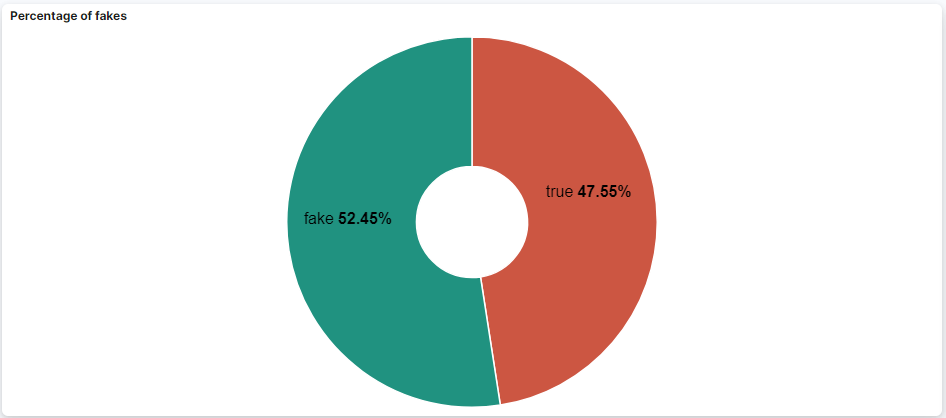
\includegraphics[width=1.0\linewidth]{Images/kibana_1.png}
  \caption{Percentage of fakes and true}
  \label{fig:kibana_1}
\end{figure}

In our dataset, the binary classification feature label distinguishing between fake and non-fake news, exhibits a well-balanced distribution (fig. \ref{fig:kibana_1}). This balance ensures that possible future models of ML are exposed to a representative mix of both classes during training. With approximately equal counts of instances labeled as fake and non-fake, we anticipate that models will be able to learn from a diverse set of examples, contributing to their generalization performance.

\newpage

\begin{figure}[h]
  \centering
  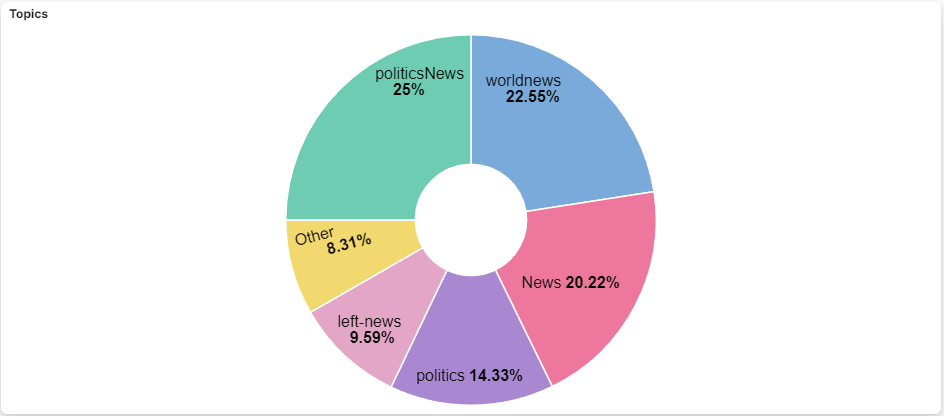
\includegraphics[width=1.0\linewidth]{Images/kibana_2.png}
  \caption{Percentage of topics}
  \label{fig:kibana_2}
\end{figure}

It's important to highlight that the naming conventions for the categories were not consistent between the labels \textbf{fake} and \textbf{true} (fig. \ref{fig:kibana_2}) (i.e. \textit{politicsNews} and \textit{politics} are redundant, or \textit{worldNews} and \textit{News}). This inconsistency in feature naming emphasizes the importance of data preprocessing and standardization to ensure uniformity in our dataset, facilitating accurate model training and evaluation.

For this reason, we have decided to merge \textit{WorldNews} with \textit{GeneralNews} and \textit{Politics News} with \textit{LeftNews} and \textit{Politics}. After this consolidation, the new distribution of categories is as follows:
\begin{itemize}
  \item Merged Politics/Left News: 53.7\%
  \item Merged World/General News: 46.3\%
\end{itemize}

\begin{figure}[h]
  \centering
  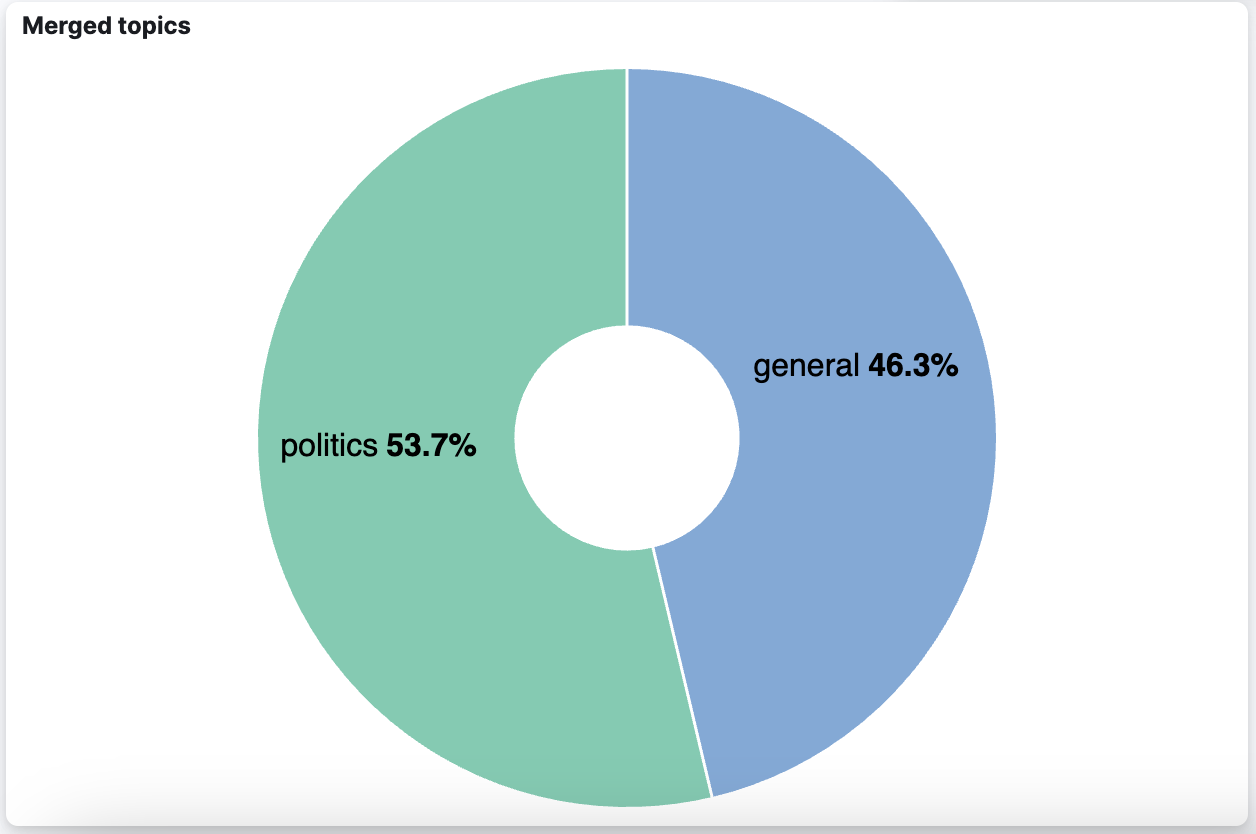
\includegraphics[width=1.0\linewidth]{Images/kibana_6.png}
  \caption{New percentage of topics}
  \label{fig:kibana_6}
\end{figure}

 This dataset covers a range of topics, with a focus on political content represented by the merged \textit{Politics/Left News} category at 53.7\%, and a significant emphasis on global and general news themes within the \textit{Merged World/General News} category, now at 46.3\%.

\newpage


\begin{figure}[h!]
  \centering
  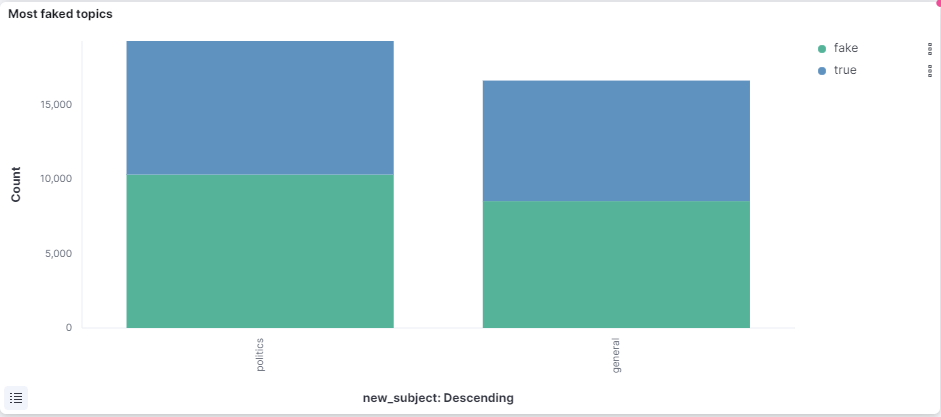
\includegraphics[width=1.1\linewidth]{Images/kibana_4.png}
  \caption{Most faked topics}
  \label{fig:kibana_4}
\end{figure}

Moreover, as expected, each topic is covered by both the \textbf{fake} and \textbf{non-fake} labels, illustrating the comprehensive representation of perspectives across different thematic categories in our dataset.
\\
\\


\begin{figure}[h]
  \centering
  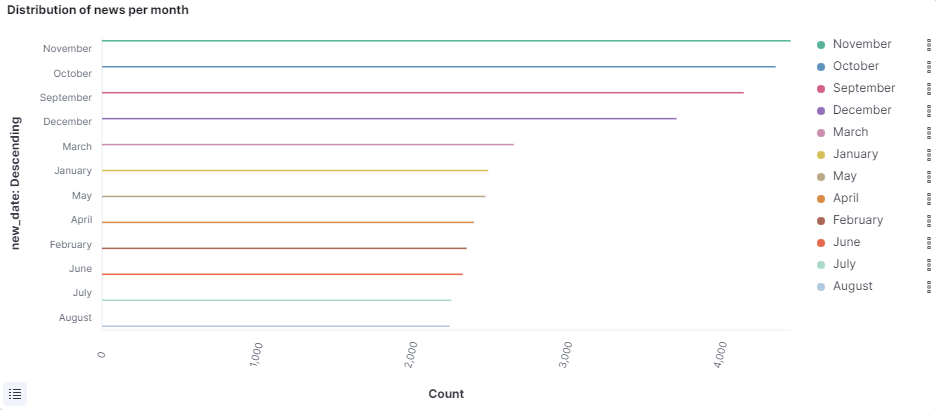
\includegraphics[width=1.0\linewidth]{Images/kibana_3.png}
  \caption{Distribution of news per month}
  \label{fig:kibana_4}
\end{figure}

Another important aspect is the frequency of news articles per month. Analyzing the distribution and trends in the number of news articles over time provides valuable insights into the dataset dynamics.

Overall, winter/fall months are the ones with highest frequency of news in our dataset. In particular, November is the month with most news and August with lowest. 

\newpage

\begin{figure}[h!]
  \centering
  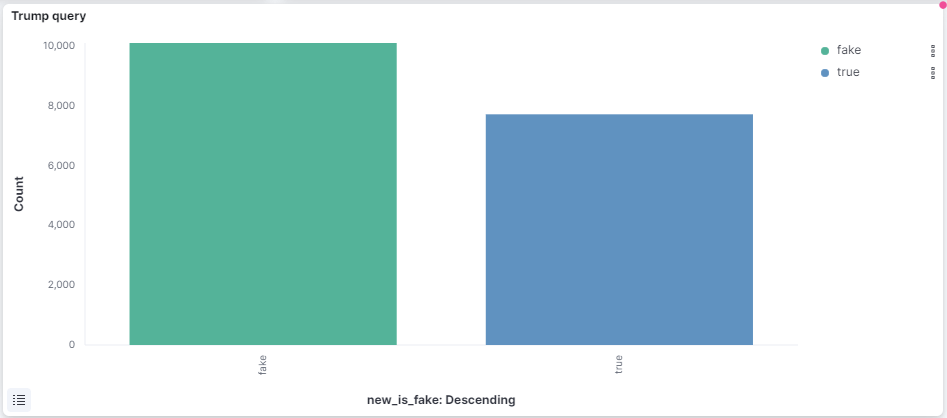
\includegraphics[width=1.0\linewidth]{Images/kibana_5.png}
  \caption{Trump results}
  \label{fig:kibana_4}
\end{figure}

An example of query regarding the difference between fake and true news is about the number of documents that contains the word "Trump".
Overall, there is an abundance of news articles about Trump, indicating a significant presence and emphasis on this topic within our dataset, but in the \textbf{fake} news category, this word is more present than in true news.



\newpage













% LIST OF FIGURES
%\listoffigures

% LIST OF TABLES
%\listoftables

%\cleardoublepage



\end{document}